\section{Results}

% Skeleton: subsection order follows the figures. Text and captions are written from numbers.md.

\subsection{Reading panels and error correlation}
% Fig. 2: panels, discussion, error correlation; panel arithmetic.

\begin{figure*}[!t]
\centering
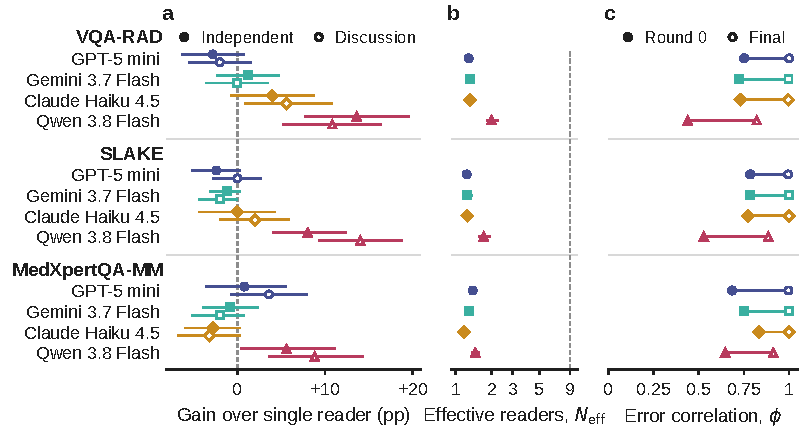
\includegraphics[width=\textwidth]{figures/fig2_panels.pdf}\\[2mm]
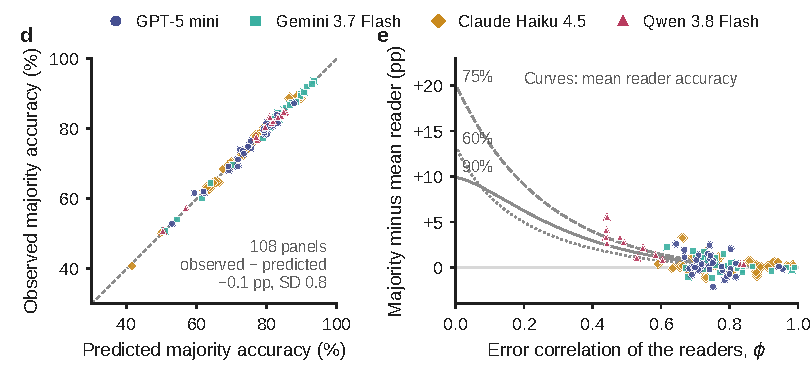
\includegraphics[width=\textwidth]{figures/fig_arithmetic.pdf}
\caption{CAPTION}
\label{fig:panels}
\end{figure*}

\subsection{Image evidence and the question-text prior}
% Fig. 3: graded evidence. Fig. 4: reader-level decomposition with the gray image; consensus errors.

\begin{figure*}[!t]
\centering
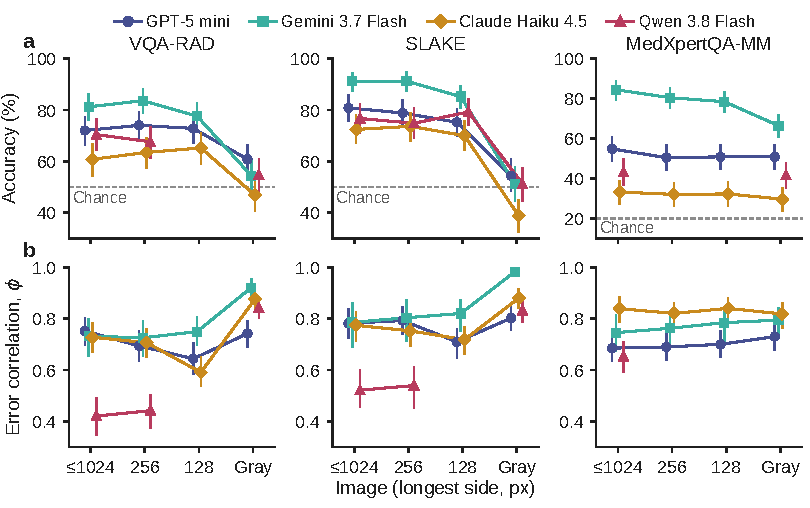
\includegraphics[width=\textwidth]{figures/fig3_evidence.pdf}
\caption{CAPTION}
\label{fig:evidence}
\end{figure*}

\begin{figure*}[!t]
\centering
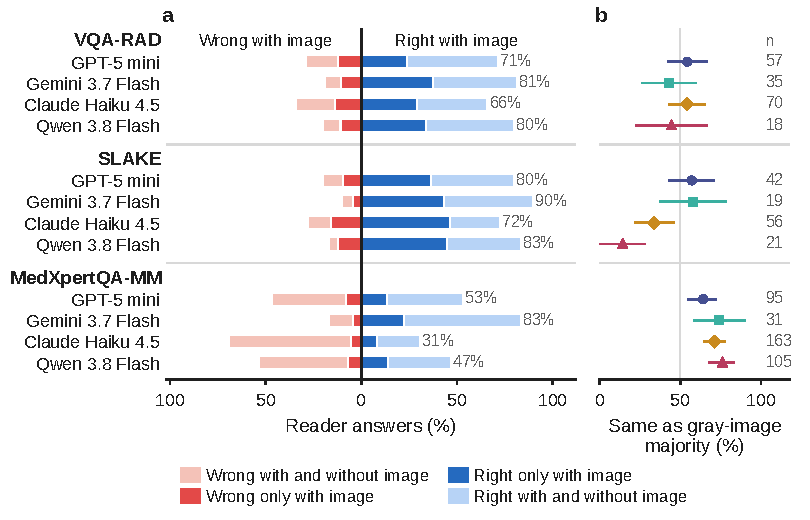
\includegraphics[width=\textwidth]{figures/fig4_prior.pdf}
\caption{CAPTION}
\label{fig:prior}
\end{figure*}

\subsection{Use of the queried region and of the image}
% Fig. 4: region occlusion; same question, different image.

\begin{figure*}[!t]
\centering
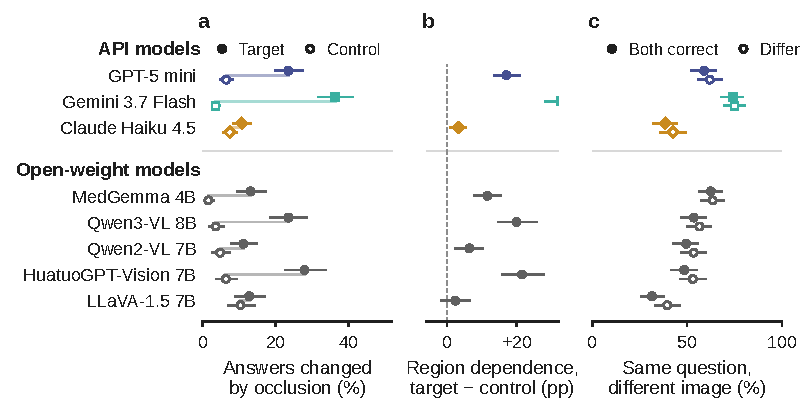
\includegraphics[width=\textwidth]{figures/fig5_region.pdf}
\caption{CAPTION}
\label{fig:region}
\end{figure*}

\subsection{Seeing and judging}
% Fig. 5: perceiver x reasoner; own and shared reports.

\begin{figure*}[!t]
\centering
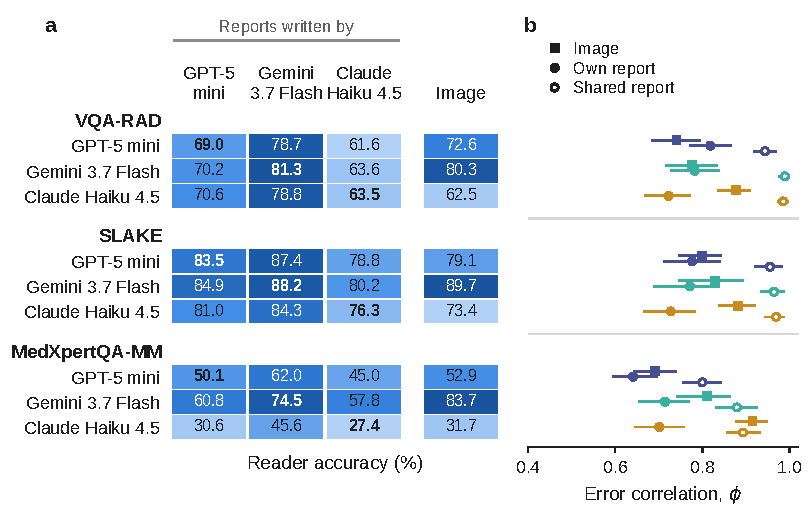
\includegraphics[width=\textwidth]{figures/fig6_report.pdf}
\caption{CAPTION}
\label{fig:report}
\end{figure*}

\subsection{What two readers share}
% Fig. 6: matched within-model contrasts.

\begin{figure*}[!t]
\centering
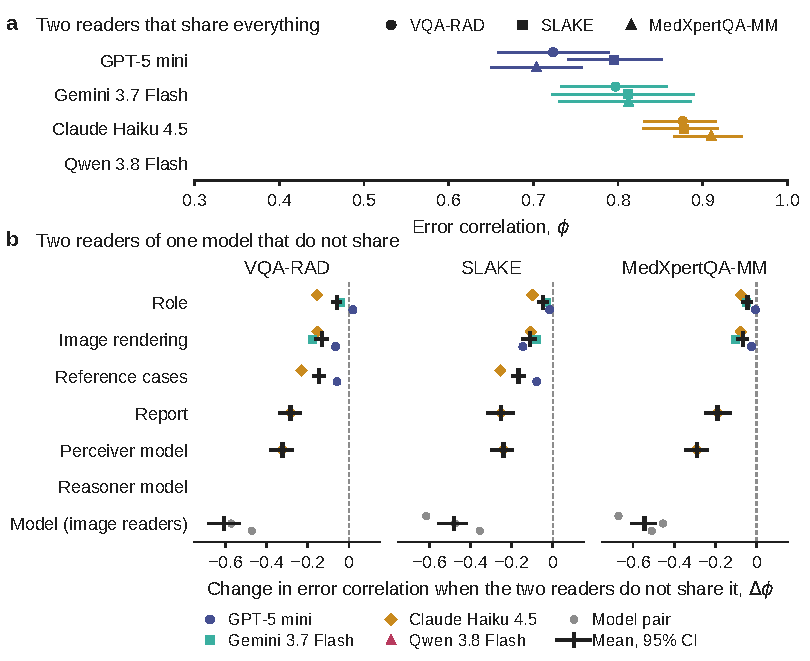
\includegraphics[width=\textwidth]{figures/fig7_budget.pdf}
\caption{CAPTION}
\label{fig:budget}
\end{figure*}

\subsection{Reference cases}
% Fig. 7: shared and private reference cases, with images or as text.

\begin{figure*}[!t]
\centering
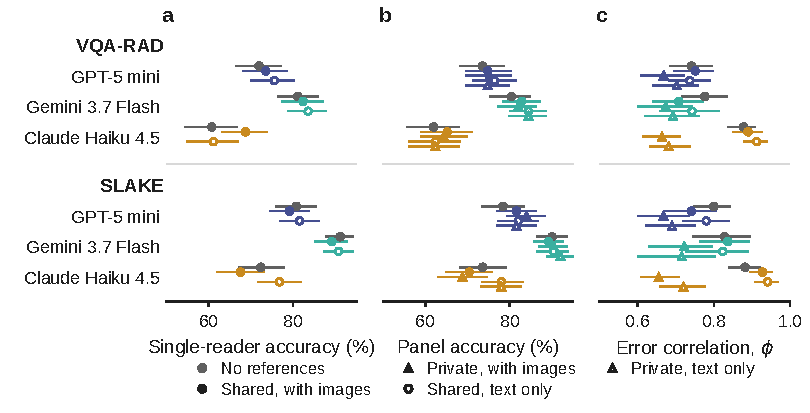
\includegraphics[width=\textwidth]{figures/fig_memory.pdf}
\caption{CAPTION}
\label{fig:memory}
\end{figure*}

\subsection{Discussion among readers}
% Fig. 8: correct round-0 answers abandoned, by origin and by round-0 position.

\begin{figure*}[!t]
\centering
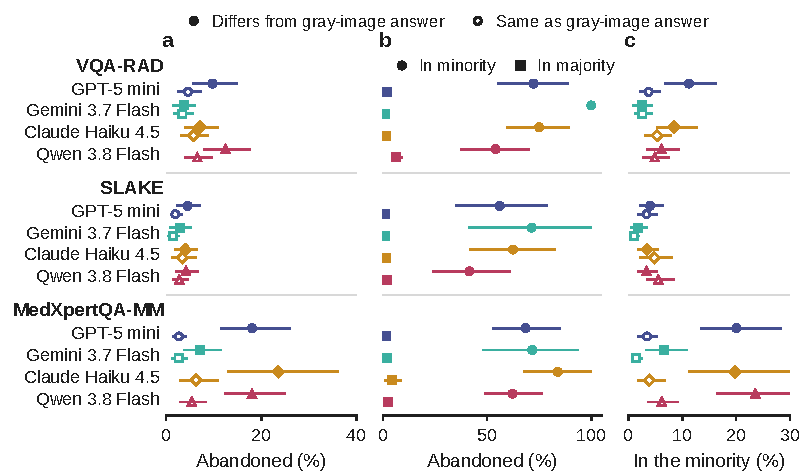
\includegraphics[width=\textwidth]{figures/fig_conformity.pdf}
\caption{CAPTION}
\label{fig:conformity}
\end{figure*}

\subsection{Open-weight models}
% Fig. S1 (supplementary): accuracy with and without the image, visual reliance, cross-model error correlation.
